\documentclass{amsart}
\usepackage{amsmath}
\usepackage{amssymb}
\usepackage{amsthm}
\usepackage{listings}
\usepackage{geometry}
\usepackage{float}
\usepackage{graphicx}
\geometry{a4paper}

\newtheorem{thm}{Theorem}
\newtheorem{prop}{Proposition}
\newtheorem{lem}{Lemma}
\newtheorem{cor}{Corollary}
\newtheorem{rem}{Remark}
\newtheorem{exa}{Example}
\newtheorem{clm}{Claim}

\theoremstyle{definition}
\newtheorem{definition}{Definition}[section]

\newtheoremstyle{case}{}{}{}{}{}{:}{ }{}
\theoremstyle{case}
\newtheorem{case}{Case}

\title{Prime Generation Draft}
\author{Jason Medcoff}
\date{}

\begin{document}
    \maketitle
    
    \begin{abstract}
    	The generation of large primes has been of great importance to modern cryptosystems. In this paper we review a widely known and deceptively efficient method for generating prime numbers: the Sieve of Eratosthenes. We build up to the algorithm with a review of some basic properties of primes and composites, and develop some results that make the sieve more efficient in practice.
    \end{abstract}
    
    % Outline
    % Intro: Review of some properties of primes
    %        fundamental theorem of arith
    %        factors less than the square root
    %        
    % Body:  The Sieve of Eratosthenes
    %        proof of the algo: correctness, time complexity
    %        code, examples
    %        Potential Improvement
    %        wheel factorization? (maybe)
    % Segmented sieve and/or sieve of Sundaram
    %
    % Conclusion
    
    
    \section{Introduction}
    
    
    
    
    \section{Some Properties of Primes and Composites}
    
%    By the Fundamental Theorem of Arithmetic, the prime numbers are demonstrated to be the key ingredients to producing the set of integers. Despite their significance, we know very little about where to find primes within the integers. Perhaps the biggest unsolved problem in mathematics today, the Riemann Hypothesis, makes a suggestion about the asymptotic distribution of the primes.

	Recall the following definition.
	\begin{definition}
		A natural number $p>1$ is said to be prime if its only positive divisors are 1 and $p$. If $p$ is not prime, it is said to be composite.
	\end{definition}
	
	One of the most important theorems with regards to the primes and integers follows.
	\begin{thm}[Fundamental Theorem of Arithmetic]\label{arith}
		If $n > 1$ is a natural number, it can be written as a product of primes unique up to the order of the factors.
	\end{thm}
	\begin{proof}
		Suppose there exists an integer $n>1$ such that $n$ cannot be written as a product of primes. By the well-ordering principle, we know that there must be a smallest $n$ satisfying this. Write $n$ as a product, $n = xy$, with $x>1$ and $y<n$. Since $n$ is the smallest positive integer that cannot be written as a product of primes, and $x$ and $y$ must be less than $n$, we can write $x$ and $y$ as products of prime factors. Then $n$ can be written as a product of primes, which contradicts the above assumption. So, every integer $n>1$ can be written as a product of primes.
		
		Next, suppose an integer $n>1$ has two prime factorizations, such that
		$$ n = j_1 \cdots j_s = k_1 \cdots k_t $$
		where all $j_i$ and $k_i$ are prime. By the well-ordering principle, we know that there must be a smallest $n$ satisfying this as well. Then $j_1 | n = k_1 \cdots k_t$ and since $j_1$ is prime, it must divide $k_i$ for some $i$. But we know that $k_i$ is prime too, so it must be that $j_1 = k_i$. Then we relabel $k_i$ as $k_1$ for simplicity, and we now cancel $j_1$ to obtain
		$$ j_2 \cdots j_s = k_2 \cdots k_t . $$
		Since $n$ is the smallest positive integer that has a non-unique prime factorization, and $ j_2 \cdots j_s = k_2 \cdots k_t < n $ is a product of primes, we arrive at a contradiction. Then there cannot exist an integer $n>1$ with two different factorizations.
	\end{proof}

	An immediate question resulting from this theorem is how we can best obtain the prime factors of arbitrary numbers. This question is still open in number theory and theoretical computer science; no classical algorithm is known that can factor a number in polynomial time on the number of digits. The difficulty of factoring very large numbers (on the order of thousands of digits) led to the creation of the RSA cryptosystem.
	
	Given some number $n$, we may want to find out whether $n$ is prime or composite. Naively, we can simply enumerate the natural numbers starting at 2, and check for divisibility, stopping when we reach $n$. However, in the interest of saving time, we can apply a result that will cut down the time spent checking divisors.
	\begin{lem}\label{sqrt}
		If $n$ is composite, at least one of its factors lies in $[2, \sqrt{n}]$.
	\end{lem}
	\begin{proof}
		Let $m = \sqrt{n}$. Then we can write $n$ as
		$$ n = m \cdot m = a \cdot b . $$
		Consider $a$. One of the following must be true: $a>m$, $a<m$, or $a=m$. In the first case, $b$ must be less than $m$; in the second case, $b$ will be greater than $m$. If $a=m$, clearly $b=m$. Therefore, if we search the integers up to $m$, we will find at least one factor of $n$.
	\end{proof}
	
	We can combine this result with the fundamental theorem of arithmetic, and easily show the following.
	\begin{cor}\label{corprime}
		Let $n>1$ be an integer. If $n$ does not have a prime factor in the range $[2, \sqrt{n}]$, it is prime.
	\end{cor}
	This is a combination of the contrapositive of lemma \ref{sqrt} with theorem \ref{arith}. So now, we have a way to check for primality of small numbers. For some $n$, we need only check divisibility by primes in $[2, \sqrt{n}]$. This algorithm, called trial division, is shown to be very slow on larger numbers. 
	
	% TODO: Prove asymptotic time complexity of trial division
	
	
	\section{Generating Primes with the Sieve of Eratosthenes}
	
	The Sieve of Eratosthenes is a process for generating primes up to some positive integer $n$. Roughly speaking, the process is to cross off the multiples of the numbers up to the square root of $n$. Those numbers that remain are the primes up to $n$.
	
	Consider the following algorithm.
	
	\begin{figure}[H]\caption{Sieve of Eratosthenes}
		\begin{lstlisting}[language=Python]
		def eratosthenes(n):
		    composites = set()
		    for i in range(2, n+1):
		        if i not in composites:
		            yield i
		            composites.update(range(i**2, n+1, i))
		\end{lstlisting}
	\end{figure}
	
	The python code above utilizes the ``set" data structure; this is suitable for two reasons. First, since we are only considering one list of numbers 2 to $n$, every element we are considering is unique, suggesting use of a set. Second, the code performs many membership checks. For lists, checking membership in a list of length $m$ is $O(m)$ in the average case, while for sets this check is $O(1)$.
	
	\begin{thm}
		The algorithm \texttt{eratosthenes} produces the prime numbers in the range $2, n$.
	\end{thm}
	\begin{proof}
		The algorithm's correctness is easy to see based on the use of \texttt{composites}. The loop invariant here is that the set \texttt{composites} contains all composite numbers between 2 and $i$; this holds for every iteration, where we yield $i$ if it is not composite, then add multiples of $i$ from $i^2$ to $n$ to the \texttt{composites} set. At the end of the last loop, every prime has been yielded in the interval $[2, n]$. Note that in addition, the algorithm is totally correct; it terminates after a finite number of steps because its loop bounds are finite.
	\end{proof}

	Informally speaking, we are using the \texttt{composites} set to ``mark" composite numbers in the range, then returning along the way those numbers which are not marked. We know that we can start at $i^2$, because all of the multiples of $i$ up to $i^2$ have already been marked off.
	
	\begin{lem}
		For every $i$ as in the algorithm above, every multiple of $i$ up to $i^2$ has already been collected into \texttt{composites}.
	\end{lem}
	\begin{proof}
		We will prove this by induction. Consider first the case of $i=2$; add it to the set \texttt{composites}. Every multiple of 2 less than $2^2 = 4$ has already been added to the set; 2 is the only such number. Then we add every multiple of 2 greater than 4 to the set, and the set contains all multiples of 2.
		Now suppose the conjecture holds for some $i=k$. Then for $i=k+1$, we consider the multiples $a(k+1)$ for some positive integer $a<k+1$. For $a=2$, we have $2k+2$, which is a multiple of 2. For $a=3$, we have a multiple of 3, and so on. For $a=k$, we have a multiple of $k$, which is already taken care of by the induction hypothesis. So every $a(k+1)$ gives a multiple of $a$. Therefore, every multiple of $i$ up to $i^2$ has been collected into \texttt{composites}.
	\end{proof}
	
	This result saves us from a lot of unnecessary set membership checking. We will now give the running time a rigorous treatment.
	
	\begin{thm}\label{runtimethm}
		The asymptotic running time of \texttt{eratosthenes} is $O(n\log\log n)$, where $n$ is the upper limit on the sieving range.
	\end{thm}
	\begin{proof}
		The noteworthy work done by the algorithm is identifying the composites; we will count these operations. For each of the $n$ iterations, we are trimming the multiples of the primes up to $n$ from the list. In particular, for $i=2$, we perform roughly $n/2$ trims, for $i=3$ we perform $n/3$, etc.\ We can write this formulation as
		$$ \sum_{p\leq n} \frac{n}{p} = n \sum_{p \leq n} \frac{1}{p} . $$
		Mertens's second theorem shows that
		$$ \lim\limits_{n\rightarrow\infty} \left[ \sum_{p \leq n} \frac{1}{p} - \log\log n - M \right] = 0 $$
		where $M$ is the Mertens constant, and rearranging terms, we observe
		$$ \lim\limits_{n\rightarrow\infty} \sum_{p \leq n} \frac{1}{p} = \lim\limits_{n\rightarrow\infty} \left[ \log\log n - M \right] . $$
		We multiply by $n$ to obtain
		$$ \lim\limits_{n\rightarrow\infty} n \sum_{p \leq n} \frac{1}{p} = \lim\limits_{n\rightarrow\infty} n \left[ \log\log n - M \right] $$
		and so the asymptotic running time as written above is
		$$ n \log \log n - nM = O(n\log\log n). $$
	\end{proof}
	
	We can concretely demonstrate the running time by writing a test. We run the algorithm some number of times, and calculate the average time taken. After performing this test for several different input sizes, we can construct a plot of running time against input size. Figure \ref{runtime1} displays the running time experiment with an average of 50 trials, on sieve sizes from 1000 to 100000. The function $f(x)$ is the result of theorem \ref{runtimethm}, multiplied by a constant. Namely, we use
	$$ f(x) = \frac{x \log \log x}{2443470.5} . $$
	
	\begin{figure}\caption{Asymptotic Running Time of \texttt{eratosthenes}}
		\label{runtime1}
		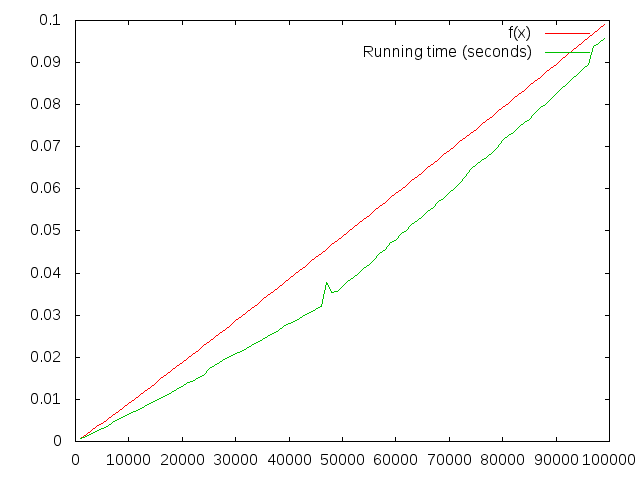
\includegraphics[scale=0.5]{erat3.png}
	\end{figure}
	
	It is evident from figure \ref{runtime1} that the function derived from the running time analysis bounds the experimental running time.


























\end{document}